\setcounter{figure}{0}
\setcounter{table}{0}
\setcounter{equation}{0}
\setcounter{section}{1}
\setcounter{subsection}{0}
\setcounter{subsubsection}{0}

\renewcommand{\thefigure}{1.\arabic{figure}}
\renewcommand{\thetable}{1.\arabic{table}}
\renewcommand{\theequation}{1.\arabic{equation}}
\renewcommand{\theHfigure}{1.\arabic{figure}}
\renewcommand{\theHtable}{1.\arabic{table}}
\renewcommand{\theHequation}{1.\arabic{equation}}
\section*{CHAPTER 1. INTRODUCTION}
\addcontentsline{toc}{section}{CHAPTER 1. INTRODUCTION}

This chapter introduces the research background and motivation behind the development of OTFS with Index Modulation (OTFS-IM) for future high-mobility wireless communication systems. The main application context of this thesis is reliable and spectrally efficient physical-layer transmission over Doppler-affected doubly selective channels, where conventional OFDM-based systems may suffer from inter-carrier interference and performance degradation. The limitations of conventional OFDM transmission are first discussed, followed by an overview of OTFS modulation, Index Modulation techniques, and related research works. Finally, the research problem, objectives, scope, methodology, and overall organization of the thesis are presented.

\subsection{Background and Motivation}


\subsubsection{Evolution of Wireless Communication Systems}

The rapid evolution of wireless communication systems has fundamentally transformed the way information is transmitted and accessed. Over the past four decades, mobile communication technologies have progressed from first-generation (1G) analog systems to modern broadband networks capable of supporting high-speed data services, multimedia applications, and massive machine-type communications. Each generation has introduced significant improvements in spectral efficiency, data rate, reliability, and network capacity.

The transition from 1G to 4G has been accompanied by major advances in waveform design and signal processing techniques. While early systems relied on frequency division multiple access (FDMA), later generations adopted time division multiple access (TDMA), code division multiple access (CDMA), and eventually orthogonal frequency division multiple access (OFDMA). As the wireless industry moves toward beyond-5G and 6G networks, waveform design must address not only higher data rates but also reliable operation in channels with stronger mobility, more severe Doppler effects, and increasingly dynamic propagation conditions.

\begin{figure}[H]
    \centering
    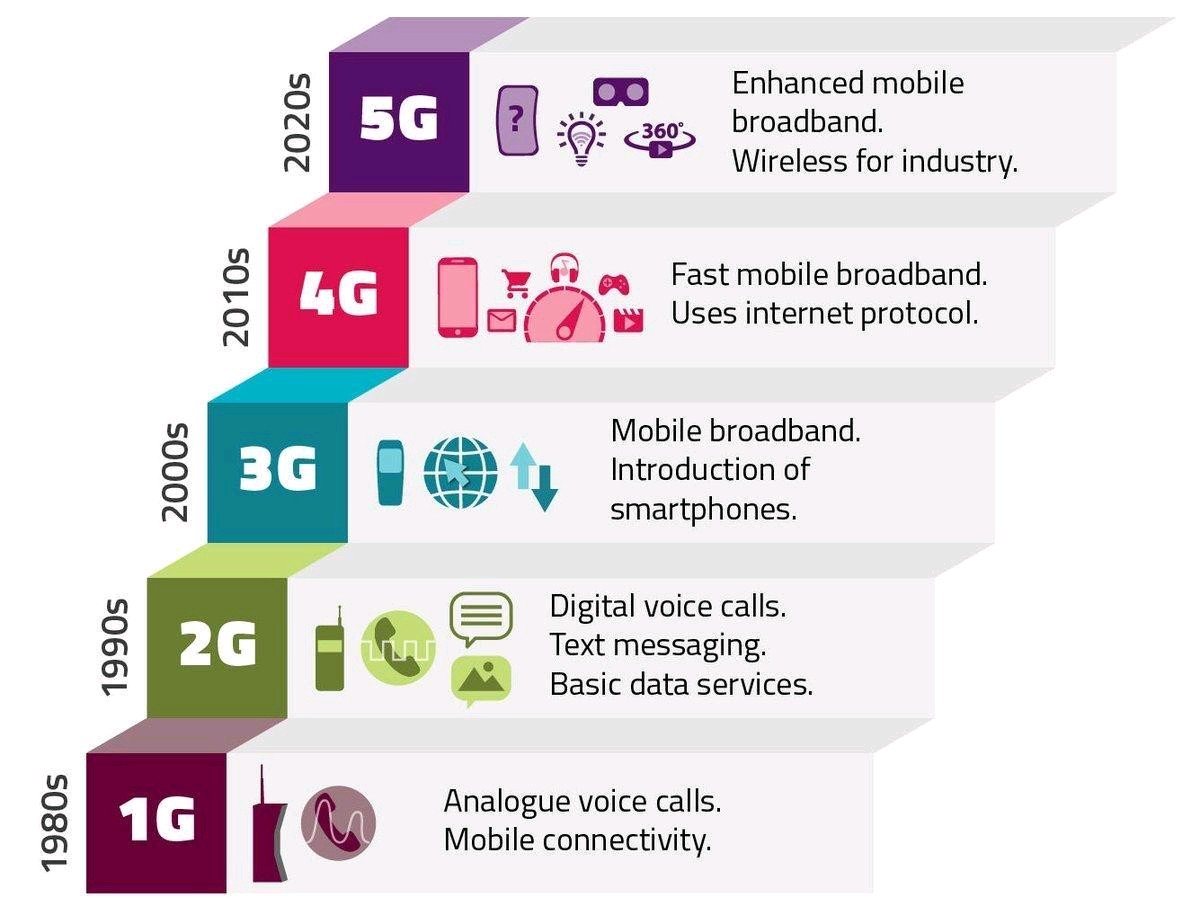
\includegraphics[width=0.75\textwidth]{Images/Chapter1/wireless_evolution.jpg}
    \caption[Evolution of wireless communication systems from 1G to 5G.]{Evolution of wireless communication systems from 1G to 5G~\protect\cite{Fig5GrowthWirelessEvolution}.}
    \label{fig:wireless_evolution}
\end{figure}

\subsubsection{Challenges in High-Mobility Communications}

Future wireless networks are expected to operate in highly dynamic environments, including high-speed trains, unmanned aerial vehicles (UAVs), vehicular communications, and low-earth-orbit satellite systems. In such scenarios, the wireless channel experiences rapid temporal variations caused by the relative motion between transmitters, receivers, and surrounding scatterers. These variations introduce significant Doppler shifts and Doppler spreads, making reliable communication increasingly challenging.

In addition to Doppler effects, multipath propagation generates delay spread due to the presence of multiple reflected signal components arriving at different times. The combined impact of delay spread and Doppler spread results in a doubly selective channel, where the channel varies across both time and frequency domains. Under these conditions, conventional communication systems often suffer from severe performance degradation because the channel characteristics change rapidly within a transmission frame.

As illustrated in Fig.~\ref{fig:ch1_channel_impairments}, multipath propagation introduces delay spread due to the existence of multiple signal propagation paths with different delays. Meanwhile, the relative motion between the transmitter, receiver, and scatterers produces Doppler spread, resulting in frequency shifts that vary among propagation paths.

\begin{figure}[H]
    \centering
    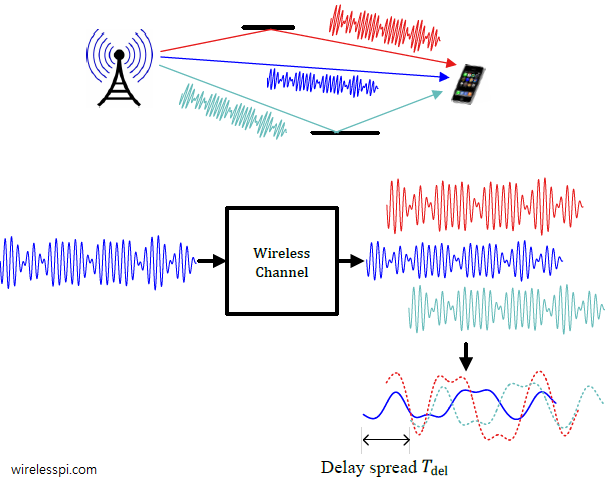
\includegraphics[width=0.8\textwidth]{Images/Chapter1/tre.png}
    \caption[Fundamental channel impairments in high-mobility wireless communications.]{Fundamental channel impairments in high-mobility wireless communications~\protect\cite{WirelessPiSmallScaleFading}.}
    \label{fig:ch1_channel_impairments}
\end{figure}

\subsubsection{Limitations of OFDM Systems}

Orthogonal Frequency Division Multiplexing (OFDM) has become the dominant modulation technique in modern wireless standards due to its ability to efficiently combat frequency-selective fading. By dividing the available bandwidth into multiple orthogonal subcarriers, OFDM converts a frequency-selective channel into a set of parallel flat-fading subchannels, allowing low-complexity one-tap equalization at the receiver.

However, the effectiveness of OFDM relies on the assumption that the wireless channel remains approximately constant during one OFDM symbol interval. In high-mobility environments, significant Doppler shifts destroy the orthogonality among subcarriers and introduce inter-carrier interference (ICI). As a result, the channel matrix loses its desirable diagonal structure, making equalization more difficult and reducing system reliability. Furthermore, the overall performance of an OFDM system is often constrained by the weakest subcarrier, leading to reduced robustness under rapidly time-varying channel conditions.

These limitations motivate the investigation of alternative waveform designs capable of operating effectively in doubly selective channels. Orthogonal Time Frequency Space (OTFS) modulation has recently emerged as a promising candidate, as it represents wireless channels in the delay-Doppler domain and provides improved resilience against high Doppler effects compared with conventional OFDM systems~\cite{Hadani2017OTFSWCNC,Hadani2018OTFS,Wei2020OTFSPromising}.

\begin{figure}[H]
    \centering
    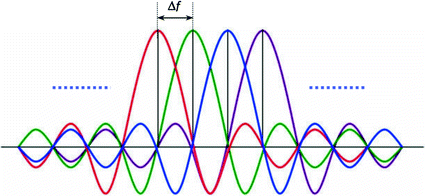
\includegraphics[width=0.75\textwidth]{Images/Chapter1/ici.png}
    \caption[Loss of subcarrier orthogonality and inter-carrier interference in OFDM under high Doppler conditions.]{Loss of subcarrier orthogonality and inter-carrier interference in OFDM under high Doppler conditions~\protect\cite{ScienceDirectICI}.}
    \label{fig:ch1_ofdm_ici}
\end{figure}

\subsubsection{Practical Application Context and Research Problem}

The practical motivation of this thesis comes from wireless links in which mobility and multipath propagation occur simultaneously. Examples include high-speed railway communications, vehicle-to-everything links, unmanned aerial vehicle communication, and satellite-assisted mobile access. In these scenarios, the received signal may contain multiple delayed replicas of the transmitted waveform, while the relative motion of terminals and scatterers introduces Doppler shifts. The resulting channel is difficult to handle with conventional time-frequency-domain designs because the channel response may vary significantly within a transmission frame.

The central physical-layer problem addressed in this thesis is therefore not only how to improve BER performance under a Doppler-affected channel, but also how to evaluate the trade-off between reliability and spectral efficiency when index-based transmission is introduced into OTFS. Baseline OTFS provides a delay-Doppler-domain modulation framework that is suitable for doubly selective channels, whereas OTFS-IM introduces additional information through the activation pattern of delay-Doppler resource elements. However, this additional flexibility also creates a design question: the selected activation patterns, the number of active positions, and the receiver detector jointly affect the final error performance.

For this reason, the thesis studies OTFS-IM as a high-mobility-inspired transmission scheme over discrete delay-Doppler channels. The goal is to evaluate how OTFS-IM behaves compared with baseline OTFS and OFDM-LMMSE references, and to examine whether distance-aware activation pattern selection can improve the reliability of index detection. This framing keeps the study close to practical high-mobility applications while remaining consistent with the MATLAB simulation model developed in the later chapters.

\subsection{Overview of OTFS and Index Modulation}

\subsubsection{Orthogonal Time Frequency Space Modulation}

Orthogonal Time Frequency Space (OTFS) modulation has recently emerged as a promising waveform candidate for future wireless communication systems operating in highly dynamic environments. Unlike conventional OFDM, which multiplexes information symbols in the time-frequency domain, OTFS maps information symbols onto the delay-Doppler domain before transmission~\cite{Hadani2017OTFSWCNC,Hong2019OTFSTutorial}. This alternative signal representation allows the wireless channel to be characterized by a small number of relatively stable propagation paths, each associated with a specific delay and Doppler shift.

The fundamental idea behind OTFS is to transform a rapidly time-varying wireless channel into a nearly invariant representation in the delay-Doppler domain. As a result, all transmitted symbols experience approximately the same channel conditions and can exploit the full time-frequency diversity available in the channel. This characteristic makes OTFS particularly attractive for high-mobility communication scenarios where conventional OFDM systems suffer from severe performance degradation.

Compared with OFDM, OTFS has demonstrated superior robustness against Doppler effects and improved reliability in doubly selective channels. Consequently, OTFS has attracted significant research interest and is considered a potential waveform candidate for beyond-5G and future 6G wireless communication systems.

\begin{figure}[H]
    \centering
    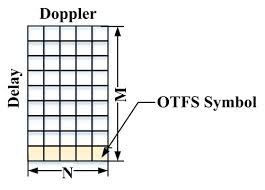
\includegraphics[width=0.88\textwidth]{Images/Chapter1/otfsframe.jpeg}
    \caption[Conceptual framework of OTFS modulation in the delay-Doppler domain.]{Conceptual framework of OTFS modulation in the delay-Doppler domain~\protect\cite{ACM3711129}.}
    \label{fig:otfs_framework}
\end{figure}

\subsubsection{Index Modulation Techniques}

Index Modulation (IM) is a transmission technique that conveys information not only through conventional modulation symbols but also through the indices of selected communication resources~\cite{Basar2016IndexMod5G,Cheng2017IndexMod5G,DoganTusha2020MultidimIM}. Depending on the system configuration, these resources may correspond to subcarriers, antennas, time slots, or other transmission entities. By exploiting additional degrees of freedom for information transmission, IM can improve spectral efficiency without requiring a proportional increase in bandwidth or transmission power.

One of the most widely studied forms of IM is Orthogonal Frequency Division Multiplexing with Index Modulation (OFDM-IM), where only a subset of subcarriers is activated during each transmission interval. The indices of the active subcarriers carry additional information bits, while the active subcarriers simultaneously transmit conventional modulation symbols. Similar concepts have also been extended to multiple-input multiple-output (MIMO) systems and various multicarrier communication frameworks.

The primary advantages of IM include improved spectral efficiency, enhanced flexibility in resource allocation, and the possibility of achieving favorable performance-complexity trade-offs. These characteristics make IM an attractive candidate for integration with advanced waveform technologies in next-generation wireless communication systems.

\begin{figure}[H]
\centering

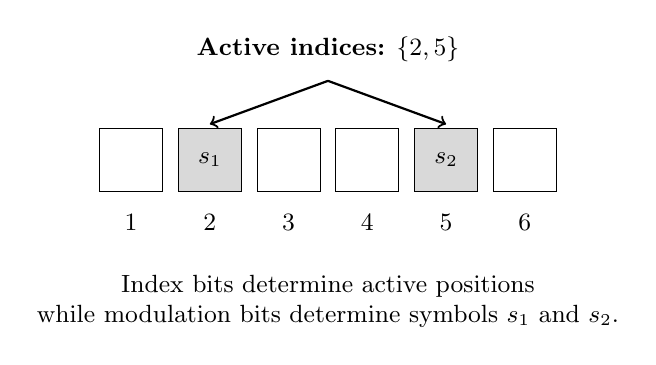
\begin{tikzpicture}[
    every node/.style={font=\small},
    active/.style={draw, fill=gray!30, minimum width=0.8cm, minimum height=0.8cm},
    inactive/.style={draw, minimum width=0.8cm, minimum height=0.8cm}
]

% Resource elements
\node[inactive] (a1) at (0,0) {};
\node[active]   (a2) at (1,0) {$s_1$};
\node[inactive] (a3) at (2,0) {};
\node[inactive] (a4) at (3,0) {};
\node[active]   (a5) at (4,0) {$s_2$};
\node[inactive] (a6) at (5,0) {};

% Index labels
\node at (0,-0.8) {1};
\node at (1,-0.8) {2};
\node at (2,-0.8) {3};
\node at (3,-0.8) {4};
\node at (4,-0.8) {5};
\node at (5,-0.8) {6};

% Text
\node[align=center] at (2.5,1.4)
{\textbf{Active indices:} $\{2,5\}$};

\node[align=center] at (2.5,-1.8)
{Index bits determine active positions\\
while modulation bits determine symbols $s_1$ and $s_2$.};

\draw[->, thick] (2.5,1.0) -- (1,0.45);
\draw[->, thick] (2.5,1.0) -- (4,0.45);

\end{tikzpicture}

\caption{Illustration of information transmission using active index patterns.}
\label{fig:index_modulation}

\end{figure}

\subsubsection{OTFS with Index Modulation}

The integration of Index Modulation into the OTFS framework leads to a new transmission scheme known as OTFS with Index Modulation (OTFS-IM). In this approach, information bits are divided into two groups. One group determines the activation pattern of delay-Doppler resource elements, while the remaining bits are mapped onto conventional constellation symbols transmitted through the activated resources.

By jointly exploiting symbol modulation and index-based information transmission, OTFS-IM can provide additional design flexibility and may improve spectral efficiency depending on the selected activation configuration. The resulting system benefits from both the delay-Doppler diversity offered by OTFS and the additional information-carrying capability introduced by IM.

Recent studies have demonstrated that OTFS-IM can achieve competitive error-rate performance while providing enhanced transmission efficiency under doubly selective fading channels. These promising characteristics motivate further investigation into the design, implementation, and performance evaluation of OTFS-IM systems, which forms the primary focus of this thesis.

\begin{figure}[H]
\centering

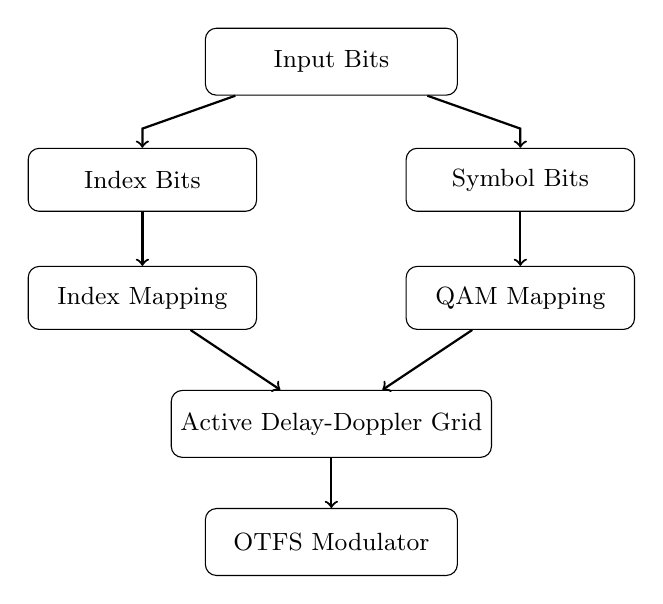
\begin{tikzpicture}[
    node distance=1.15cm,
    every node/.style={font=\small},
    block/.style={
        draw,
        rounded corners,
        minimum width=3.2cm,
        minimum height=0.85cm,
        align=center
    },
    smallblock/.style={
        draw,
        rounded corners,
        minimum width=2.9cm,
        minimum height=0.8cm,
        align=center
    },
    arrow/.style={->, thick}
]

% Main input
\node[block] (bits) at (0,0) {Input Bits};

% Split branches
\node[smallblock] (indexbits) at (-2.4,-1.5) {Index Bits};
\node[smallblock] (symbolbits) at (2.4,-1.5) {Symbol Bits};

\node[smallblock] (indexmap) at (-2.4,-3.0) {Index Mapping};
\node[smallblock] (qammap) at (2.4,-3.0) {QAM Mapping};

% Merge
\node[block] (ddgrid) at (0,-4.6) {Active Delay-Doppler Grid};

\node[block] (otfs) at (0,-6.1) {OTFS Modulator};

% Arrows
\draw[arrow] (bits) -- (-2.4,-0.85) -- (indexbits);
\draw[arrow] (bits) -- (2.4,-0.85) -- (symbolbits);

\draw[arrow] (indexbits) -- (indexmap);
\draw[arrow] (symbolbits) -- (qammap);

\draw[arrow] (indexmap) -- (ddgrid);
\draw[arrow] (qammap) -- (ddgrid);

\draw[arrow] (ddgrid) -- (otfs);

\end{tikzpicture}

\caption{Basic principle of information transmission in an OTFS-IM system.}
\label{fig:otfs_im_concept}

\end{figure}

\subsection{Related Works}

Research on high-mobility wireless transmission has shown that conventional OFDM can suffer from severe inter-carrier interference when Doppler effects are strong~\cite{Hadani2017OTFSWCNC,Wei2020OTFSPromising,Raviteja2018OTFSInterference}. Although OFDM remains attractive because of its simple FFT-based implementation and low-complexity equalization, its performance depends heavily on the preservation of subcarrier orthogonality. This limitation has motivated the study of alternative modulation schemes that are more suitable for doubly selective channels.

OTFS was introduced as a delay-Doppler-domain modulation technique to improve robustness in time-varying channels~\cite{Hadani2017OTFSWCNC,Hadani2018OTFS,Wei2020OTFSPromising,Hong2019OTFSTutorial}. Later works further analyzed OTFS input-output relations, interference behavior, and receiver design, including message passing and linear equalization methods~\cite{Raviteja2018OTFSMP,Raviteja2018OTFSInterference,Surabhi2020LinearEqualization}. These studies indicate that representing the channel in the delay-Doppler domain can provide a more stable structure for high-mobility communication than conventional time-frequency-domain processing.

In parallel, Index Modulation has been widely studied as a method for transmitting extra information through the indices of active resources~\cite{Basar2016IndexMod5G,Cheng2017IndexMod5G,DoganTusha2020MultidimIM}. OFDM-IM is a representative example, where only a subset of subcarriers is activated and the active-subcarrier pattern carries additional bits~\cite{Wen2017OFDMIM}. This principle can improve flexibility in the trade-off among reliability, spectral efficiency, and detection complexity.

Recent studies have extended the IM concept to OTFS systems and reported that OTFS-IM can achieve promising BER and spectral-efficiency performance over doubly selective channels~\cite{Liang2020OTFSIM,Qian2022BlockWiseOTFSIM,Qian2023ReceiverOTFSIM,Wu2024OTFSIMDetector}. However, the final performance of OTFS-IM depends strongly on activation-pattern design, the number of active delay-Doppler positions, and the receiver detection method. Therefore, this thesis focuses on a simulation-based evaluation of OTFS-IM, with particular attention to distance-aware activation-pattern selection and the decomposition of total BER into index and symbol error components. This provides the basis for the research objectives and methodology presented in the following section.

\subsection{Research Objectives and Methodology}

\subsubsection{Research Objectives}

The primary objective of this thesis is to investigate the applicability of Orthogonal Time Frequency Space modulation combined with Index Modulation techniques for high-mobility-inspired wireless communication environments. The study focuses on analyzing the performance characteristics of OTFS-IM systems and evaluating their potential advantages and limitations compared with conventional OTFS transmission schemes.

To achieve this objective, the theoretical foundations of OTFS modulation and Index Modulation are first studied in detail. Particular attention is given to the representation of wireless channels in the delay-Doppler domain, which forms the basis for the robustness of OTFS under rapidly time-varying channel conditions. Furthermore, the principles of index-based information transmission are investigated to understand how additional information can be conveyed through the activation patterns of transmission resources.

Based on these theoretical foundations, an OTFS-IM transmission framework is developed and implemented in MATLAB. The proposed system is evaluated under doubly selective fading channels with various signal-to-noise ratios. The performance of the system is assessed primarily in terms of Bit Error Rate (BER), while the impact of different index activation patterns, modulation parameters, and spectral-efficiency configurations is also examined.

The final objective of the thesis is to provide a comprehensive performance evaluation of OTFS-IM and to identify its potential benefits and limitations for future high-mobility wireless communication systems. The obtained results are expected to contribute to the ongoing development of waveform technologies for beyond-5G and sixth-generation (6G) communication networks.

\subsubsection{Main Contributions of the Thesis}

The first contribution of this thesis is the development of a MATLAB-based simulation framework for comparing OFDM-LMMSE, baseline OTFS, and OTFS-IM under a common delay-Doppler channel model. This framework allows the effect of Doppler-aware signal representation and index-based transmission to be evaluated within the same physical-layer setting.

The second contribution is the construction and evaluation of an OTFS-IM transmission chain in which information bits are divided into index bits and constellation bits. Different activation configurations are considered in order to study how the number of active positions affects BER performance and spectral efficiency. This is important because OTFS-IM does not always improve all performance metrics simultaneously; instead, it introduces a reliability-efficiency trade-off that must be analyzed carefully.

The third contribution is the investigation of activation-pattern selection strategies for OTFS-IM. In particular, Hamming-distance-aware pattern selection and its balanced variant are examined as rule-based methods for selecting delay-Doppler activation patterns. These methods are compared with random pattern selection to assess whether larger pairwise pattern separation and more balanced carrier usage can improve index detection reliability.

The final contribution is a multi-level performance analysis that includes total BER, index BER, symbol BER, pattern error rate, and BER-spectral-efficiency trade-off across several OTFS-IM configurations. Instead of relying on a single BER curve, the thesis analyzes where the performance gain or loss originates, thereby providing a clearer interpretation of the behavior of OTFS-IM systems under the considered simulation assumptions.

\subsubsection{Research Scope}

This thesis focuses on the investigation of OTFS modulation and OTFS with Index Modulation under high-mobility-inspired wireless communication scenarios. The study is limited to single-user transmission systems and considers doubly selective fading channels characterized by both delay spread and Doppler spread.

The research primarily concentrates on the physical layer aspects of wireless communication systems. Channel coding, medium access control protocols, resource scheduling, and higher-layer networking issues are beyond the scope of this work. Instead, emphasis is placed on signal modulation, index mapping strategies, delay-Doppler domain processing, and receiver detection techniques.

A simulation-based approach is adopted throughout the study. The performance evaluation is carried out using MATLAB-based implementations of both conventional OTFS and OTFS-IM systems. The considered performance metric is the Bit Error Rate (BER), which is evaluated under different signal-to-noise ratio conditions. Various system parameters, including modulation order and index activation configurations, are investigated to analyze their influence on system performance.

It should be noted that practical implementation issues such as hardware impairments, synchronization errors, channel estimation inaccuracies, and real-time processing constraints are not explicitly addressed in this thesis. These aspects are left for future research and experimental validation.

\subsubsection{Research Methodology}

The research methodology adopted in this thesis consists of four main stages, including theoretical analysis, system modeling, simulation implementation, and performance evaluation.

The first stage involves an extensive review of the existing literature related to wireless communication systems operating in high-mobility environments. Particular attention is given to the theoretical principles of OTFS modulation, delay-Doppler domain channel representation, and Index Modulation techniques. Relevant research articles, tutorial papers, and recent survey studies are examined to establish a comprehensive theoretical foundation for the proposed work.

The second stage focuses on the development of mathematical models for both OTFS and OTFS-IM systems. The signal processing procedures involved in transmission and reception are analyzed, including symbol mapping, index selection, delay-Doppler domain modulation, channel propagation, and receiver detection. These models provide the basis for the simulation framework employed throughout the study.

The third stage consists of implementing the developed models in MATLAB. The simulation environment is designed to emulate high-mobility wireless channels with varying Doppler conditions and additive white Gaussian noise. Different system configurations are considered to investigate the influence of modulation parameters and index activation strategies on communication performance.

The final stage involves analyzing and comparing the obtained simulation results. The BER performance of conventional OTFS and OTFS-IM systems is evaluated over a range of signal-to-noise ratios. Based on the observed results, conclusions are drawn regarding the effectiveness of index modulation in improving the performance and transmission efficiency of OTFS systems under challenging wireless channel conditions.

\begin{figure}[H]
    \centering
    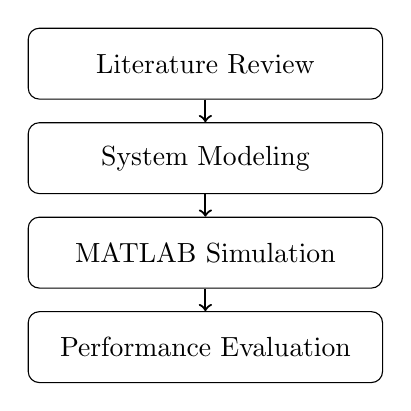
\begin{tikzpicture}[
        node distance=1.2cm,
        block/.style={
            draw,
            rounded corners,
            minimum width=4.5cm,
            minimum height=0.9cm,
            align=center
        },
        arrow/.style={->, thick}
    ]

    \node[block] (lit) {Literature Review};

    \node[block, below of=lit] (model) {System Modeling};

    \node[block, below of=model] (sim) {MATLAB Simulation};

    \node[block, below of=sim] (eval) {Performance Evaluation};

    \draw[arrow] (lit) -- (model);
    \draw[arrow] (model) -- (sim);
    \draw[arrow] (sim) -- (eval);

    \end{tikzpicture}

    \caption{Research methodology adopted in this thesis.}
    \label{fig:research_methodology}
\end{figure}

\subsection{Thesis Organization}

The remainder of this thesis is organized as follows.

Chapter 2 presents the theoretical background required for understanding the proposed system. Fundamental concepts of wireless communication channels, multipath propagation, Doppler effects, Orthogonal Frequency Division Multiplexing (OFDM), delay-Doppler domain representation, and Index Modulation techniques are reviewed. The limitations of conventional multicarrier systems in high-mobility environments are also discussed.

Chapter 3 introduces the principles of Orthogonal Time Frequency Space (OTFS) modulation. The OTFS transmitter and receiver structures, delay-Doppler domain signal representation, modulation and demodulation processes, and input-output relationships are presented. The advantages of OTFS over conventional OFDM systems in doubly selective channels are also analyzed.

Chapter 4 focuses on the integration of Index Modulation into the OTFS framework. The operating principles of OTFS-IM, index mapping strategies, resource activation patterns, transmitter and receiver architectures, and detection mechanisms are described. Furthermore, the expected benefits and design considerations of OTFS-IM systems are discussed.

Chapter 5 presents the simulation framework and performance evaluation of the proposed systems. MATLAB-based implementations of OTFS and OTFS-IM are developed and tested under various channel conditions. The performance of the considered schemes is evaluated primarily in terms of Bit Error Rate (BER), and comparisons are conducted to investigate the impact of different system parameters and index activation configurations.

Finally, Chapter 6 summarizes the main findings of the thesis and highlights the key contributions of the conducted research. Possible directions for future work and further improvements of OTFS-IM systems are also suggested.

\begin{figure}[H]
    \centering
    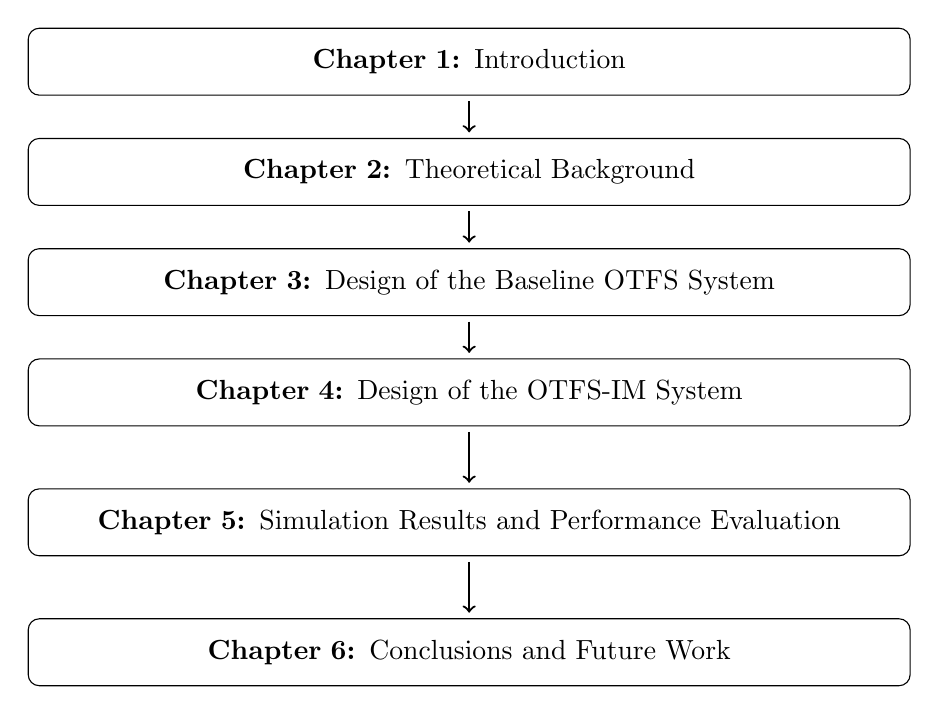
\begin{tikzpicture}[
        block/.style={
            draw,
            rounded corners,
            minimum width=11.2cm,
            minimum height=0.85cm,
            text width=10.4cm,
            align=center,
            inner sep=6pt
        },
        arrow/.style={->, thick, shorten >=2pt, shorten <=2pt}
    ]

    \node[block] (c1) at (0,0) {\textbf{Chapter 1:} Introduction};
    \node[block] (c2) at (0,-1.40) {\textbf{Chapter 2:} Theoretical Background};
    \node[block] (c3) at (0,-2.80) {\textbf{Chapter 3:} Design of the Baseline OTFS System};
    \node[block] (c4) at (0,-4.20) {\textbf{Chapter 4:} Design of the OTFS-IM System};
    \node[block] (c5) at (0,-5.85) {\textbf{Chapter 5:} Simulation Results and Performance Evaluation};
    \node[block] (c6) at (0,-7.50) {\textbf{Chapter 6:} Conclusions and Future Work};

    \draw[arrow] (c1) -- (c2);
    \draw[arrow] (c2) -- (c3);
    \draw[arrow] (c3) -- (c4);
    \draw[arrow] (c4) -- (c5);
    \draw[arrow] (c5) -- (c6);

    \end{tikzpicture}

    \caption{Thesis structure and chapter progression.}
    \label{fig:thesis_organization}
\end{figure}

The structure presented in Fig.~\ref{fig:thesis_organization} illustrates the logical flow of the research conducted in this thesis. The organization begins with the research motivation and theoretical background, followed by the baseline OTFS system design and the OTFS-IM extension. The developed systems are then evaluated through simulation, and the final chapter summarizes the main findings, limitations, and future research directions.

\newpage
